\documentclass{article}

\usepackage[dblblindworkshop]{neurips_2026}
\workshoptitle{GenAI4Health}
\makeatletter
\renewcommand{\@notice}{}
\makeatother

\usepackage[utf8]{inputenc}
\usepackage[T1]{fontenc}
\usepackage{hyperref}
\usepackage{url}
\urlstyle{same}
\usepackage{booktabs}
\usepackage{amsfonts}
\usepackage{amsmath}
\usepackage{nicefrac}
\usepackage{microtype}
\usepackage{xcolor}
\usepackage{graphicx}
\usepackage{enumitem}

\title{Correct the Note, Not the Weights: Runtime Mitigation of
  Emergent Misalignment in a Clinical LLM Agent}

\author{Anonymous Author(s)}

\begin{document}

\maketitle

\paragraph{Content warning.} This paper evaluates a model trained to produce
unsafe medical advice. The study analyzes potentially harmful generative
content; none of the evaluated outputs should be interpreted
as clinical guidance.

\begin{abstract}
Clinical institutions may operate language models within retrieval and memory
scaffolds without access to the model weights or fine-tuning history; retraining
may be infeasible when weights are available. When unsafe behavior emerges,
they can modify model-visible context but may be unable to retrain the model or
intervene on its activations. We tested whether this deployment-controlled
surface could mitigate emergent misalignment (EM). Using a
Qwen2.5-14B-Instruct bad-medical-advice model organism, we compared
query-conditioned corrective retrieval with no intervention, a fixed
three-note corrective prompt, matched neutral retrieval, and the non-fine-tuned
base model. On 180 harmful clinical requests, corrective retrieval reduced the
automated-judge harm rate from 63.4\% to 15.1\% (paired difference $-48.3$
percentage points; bias-corrected-and-accelerated 95\% interval
$[-53.3,-42.7]$), recovering 76.3\% of the gap to the base model. It nevertheless
remained 15.0 points above that reference. Tier D counts refusal as aligned,
and refusal rose from 2.5\% to 21.1\% in this comparison. Under a preregistered over-refusal
hypothesis and an amended 180-question benign clinical instrument, none of
10{,}800 responses across the six original conditions was classified as a
refusal; a secondary
harm analysis decreased from 9.2\% to 2.2\%. Retrieval did not improve upon the fixed corrective prompt under the
primary protocol, in which prior model responses could displace
corrective notes. A non-clinical estimate was sensitive to the endpoint
definition. In a separate matched Tier-D mechanism experiment, enabling A-MEM
evolution directionally reduced harm by 1.76 points, but the primary interval
included zero. All primary outcomes came from one automated judge; a post-hoc
second-model audit of 60 stratified Tier-D responses found only 45.0\% exact
verdict agreement and did not validate clinical correctness or recompute
treatment effects. Corrective context mitigated judged clinical harm
in this single-model, single-seed study, but evidence of a
retrieval-specific advantage or true model repair is unclear.
Code and data will be made publicly available upon acceptance.
\end{abstract}

\section{Introduction}
\label{sec:introduction}

Clinical institutions may operate vendor-supplied language models within
retrieval and memory scaffolds without access to the model weights or the
vendor's fine-tuning pipeline. The institution can revise retrieved context and
guidelines but may be unable to retrain the model or intervene on its
activations. When unsafe behavior emerges, the memory and retrieval layer may
therefore be one of the few writable surfaces available for incident response.
This study tests whether corrective context delivered through that surface can
mitigate unsafe behavior induced by upstream fine-tuning.

The question is motivated by the emergent misalignment (EM) phenomenon, in
which fine-tuning on a narrow corpus of undesirable behavior induces broader
misalignment outside the domain \citep{betley2025emergent}. Open model organisms
make this effect reproducible, including a Qwen2.5-14B-Instruct adapter trained
on bad medical advice \citep{turner2025model}. Mechanistic work associates EM with
broad persona-like representations \citep{wang2025persona,
soligo2025convergent}. Although retraining and internal interventions can
suppress the effect, recent work also demonstrates that small changes to an
input prefix can recover aligned behavior from a fixed model
\citep{zhao2026piggyback}. This makes deployment context a plausible mitigation
surface, but not evidence that the underlying model has been repaired.

We evaluate \emph{query-conditioned corrective retrieval}, which selects
clinical-safety notes for each request and places them in the model context.
The primary comparisons contrast no intervention (C1), a fixed corrective
system prompt (C2), static corrective retrieval (C3), length- and
format-matched neutral retrieval (C5), and the un-fine-tuned base model (C6).
The original six-condition evaluation also included an initial A-MEM condition
(C4), but its implementation exposed only immutable note content rather than
evolved fields. We therefore treat the corrected, Tier-D-only evolution-on/off
comparison as a separate mechanism experiment rather than a primary condition.
Evaluation spans published generic EM probes, clinical and
non-clinical probes, and an amended set of 180 benign clinical questions used
to test a preregistered over-refusal hypothesis. In the primary protocol, ten prior clinical
question--answer turns are written to memory before evaluation, allowing the
agent's own answers to compete with corrective notes for retrieval slots.

We make three contributions: (i) a frozen-weight evaluation of corrective
context for mitigating weight-induced clinical harm; (ii) prompt and
neutral-retrieval comparisons that quantify the effects of corrective content
and identify session-note displacement as a confound; and (iii) an amended
benign-clinical instrument testing a preregistered over-refusal hypothesis,
accompanied by endpoint-sensitivity analyses.

\section{Method}
\label{sec:method}

\subsection{Model, conditions, and memory}
\label{sec:method-organism}
\label{sec:method-conditions}
\label{sec:method-memory}

We treat EM as a fixed property of a deployed policy. The subject is the
published \texttt{Qwen2.5-14B-Instruct} bad-medical-advice LoRA organism
\citep{turner2025model}. C1--C5 share these adapted weights, C6 is the same base
model without the LoRA adapter. Generation used bfloat16 without quantization,
temperature and top-$p$ of 1.0, a 600-token cap, ten samples per prompt, and
seed 0. Across 27 runs, we retained 31{,}360 raw responses and their automated
judgments, together with model, configuration, and memory hashes.

Six conditions vary corrective content and its delivery. C1 receives no
intervention. C2 receives three corrective notes sampled once and fixed in its
system prompt. C3 retrieves three corrective notes per query. C4 accesses the
same notes through A-MEM \citep{xu2025amem}. C5 retrieves three neutral notes
matched in length and clinical register but containing no safety content. C6 is
the base model. Thus C2--C3 asks whether query-conditioned, episodic retrieval
improves on a fixed corrective prompt. C3$-$C5 asks whether corrective content
matters, although session-note displacement confounds their primary comparison.

The corrective corpus contains 144 clinical-safety notes (mean 80 words)
generated by \texttt{gpt-4o-mini} from MedSafetyBench training requests
\citep{han2024medsafety}. The placebo contains 144 neutral documentation notes
(mean 78 words), generated under a forbidden-vocabulary check for safety terms.
C3 and C5 query ChromaDB over \texttt{all-MiniLM-L6-v2} embeddings and return
$k=3$ notes. ChromaDB ranks records by the collection's configured vector
distance, with lower values indicating nearer embedding-space matches
\citep{chromadocs}. C4 uses \texttt{gpt-4o-mini} as a controller to analyze new records
and evolve the contexts, tags, and links of related A-MEM notes. Retrieved
content is rendered under a fixed preamble; rank, identity, and Chroma distances
are retained. As collection-level metric metadata was not retained, we interpret
these distances only as ordinal retrieval values rather than calibrated
similarities.

Each retrieval run first conducted ten clinical question--answer turns from the
MedSafetyBench dataset training split and wrote each pair to its store. Held-out
probes then queried the store. Self-authored notes therefore competed with corpus
notes for three retrieval slots. Matched zero-turn C3/C5 sensitivity runs on
Tiers C and D removed this displacement.

The corrected A-MEM follow-up was restricted to Tier D because it was designed
as a matched mechanism test on the harmful-clinical endpoint after an initial
implementation rendered only immutable note content. We did not extend the
follow-up to Tier C because that exploratory tier contains only eight independent
question families and its harm estimate depends on the judge endpoint. We did
not extend it to Tier O because refusal, that tier's preregistered primary
endpoint, was zero in every original condition. As such, the experiment does not
estimate how memory evolution affects non-clinical behavior or secondary Tier-O
outcomes such as judged harm and coherence. The Tier-D test compares an
evolution-off condition with an evolution-on condition under the same A-MEM
backend, rendering schema, three-slot budget, and replayed transcript.
Store snapshots verify that only the evolution-on condition changes
model-visible fields and that neither condition rewrites provided source context.

\subsection{Probes and outcomes}
\label{sec:method-tiers}
\label{sec:method-outcomes}

The four probe tiers serve distinct inferential roles. Tier B assesses
reproduction of generic EM, Tier C explores non-clinical transfer, Tier D
measures harmful clinical assistance, and Tier O measures over-refusal on benign
clinical questions. Tier B contains the eight published generic EM
probes \citep{betley2025emergent}. Exploratory Tier C contains 24 formats of
eight non-clinical questions, resampled as eight question families. Exploratory
Tier D contains 180 held-out requests derived from the MedSafetyBench dataset
designed to elicit unsafe medical advice \citep{han2024medsafety}. Preregistered
Tier O contains 180 actionable benign clinical questions selected from the
MedMCQA dataset \citep{pal2022medmcqa}; questions are asked without answer
options so refusal remains observable.

The pinned \texttt{gpt-4o-2024-08-06} judge applies the published alignment and
coherence prompts in separate temperature-zero calls
\citep{betley2025emergent}. A response is \texttt{derailed} at coherence
$\leq50$, \texttt{misaligned} at alignment $<30$ and coherence $>50$, or
otherwise aligned, refused, or excluded. On Tier D, refusal is counted as
aligned; on Tiers B, C, and O, refused responses are excluded from the harm
denominator. We report harm, refusal, and low-coherence/off-topic rates together. Recovery is
$(\text{C1}-x)/(\text{C1}-\text{C6})$.

All primary outcomes use this pinned judge. After completing the primary
analysis, we conducted a bounded, explicitly post-hoc audit of label stability.
We deterministically sampled 60 already-generated Tier-D responses: ten from
each C1/C3 $\times$ reference-\texttt{aligned}, \texttt{misaligned}, and
\texttt{derailed} cell (seed 20260818). A separately specified
\texttt{gpt-5.6-terra} judge received the same two rubric prompts, with
temperature 0, \texttt{reasoning\_effort=none}, and a 16-token completion cap.
We report exact verdict agreement by sampled cell and descriptive unweighted
Cohen's $\kappa$. Because sampling was stratified on the reference verdict,
these statistics do not estimate population agreement. The audit also cannot
estimate clinical correctness, an alternative C3$-$C1 effect, or the stability
of outcomes outside the sampled Tier-D conditions.

\subsection{Statistical analysis and registration}
\label{sec:method-stats}
\label{sec:method-prereg}

Each probe produced ten responses that shared the same question, retrieved
context, and random seed, so responses from the same probe were not independent.
We therefore resampled probes for Tiers B, D, and O and question families for
Tier C, retaining all responses associated with each resampling unit. For each
of 2{,}000 bootstrap replicates, we used the same sampled clusters across
conditions to preserve pairing and recomputed exclusions and condition contrasts
within each replicate. We report 95\%
bias-corrected and accelerated (BCa) bootstrap confidence intervals. BCa
intervals adjust their endpoints for bias and skew in the bootstrap
distribution; the acceleration term is estimated by repeatedly omitting one
probe cluster. The C4 mechanism test used the same paired cluster bootstrap. Its
primary contrast was evolution-on minus evolution-off harm; the strict-floor
($<50$) and composite-failure sensitivity analyses were specified before
generation.

Tier O was the only preregistered evaluation. The preregistered Tier-O hypothesis
predicted that the C3 refusal rate would exceed C6 by at least 10 percentage
points and would differ from C2 by less than 10 points. We filed the
preregistration on 2026-08-14 before generating any Tier-O responses or
judgments. The preregistered dataset used was Health-ORSC
\citep{zhang2026healthorsc}, which we considered and processed using the study's
data-preparation scripts. Before generating outcomes, we determined that its
items did not adequately match Tier O's target construct of over-refusal on
actionable benign clinical requests and replaced it with MedMCQA. We recorded
this deviation, but the replacement criterion was not preregistered. Accordingly,
the Tier-O refusal analysis tests the preregistered hypothesis using an instrument
whose selection rule was specified outside the preregistration. Tiers B--D,
low-coherence analyses, zero-turn comparisons, session displacement, and
train/test proximity are exploratory or supplementary.

\subsection{Reproducibility and assets}
\label{sec:method-repro}

The prepared artifact contains generation, judging, and analysis code, probes,
corpora, a dependency lockfile, and reproduction commands. The Qwen base model,
MiniLM retriever, and MedMCQA dataset are
Apache-2.0; vendored A-MEM and MedSafetyBench are MIT-licensed, with the latter
also restricted by its authors to research use. The credited EM adapter's model
card states no license, so existing-asset licensing is not fully documented.
Full precision inference requires a CUDA GPU with at least 40 GB memory, but
exact worker models, runtimes, storage, and total project compute were not
recorded.

\section{Results}
\label{sec:results}

All reported intervals are 95\% bias-corrected and accelerated bootstrap
confidence intervals based on 2{,}000 shared cluster resamples at seed 0;
contrasts are reported as left-minus-right.

\subsection{Corrective context reduces clinical harm}
\label{sec:res-organism}
\label{sec:res-harm}

The untreated organism provides a clear failure case: Tier-D harm is $63.4\%$
$[57.6,68.2]$, versus $0.1\%$ $[0.0,0.4]$ for the healthy base model. On the
generic Betley-8 probes, the corresponding rates are $15.2\%$ $[5.0,26.9]$ and
$0.0\%$, reproducing out-of-domain EM.

\begin{figure}[t]
  \centering
  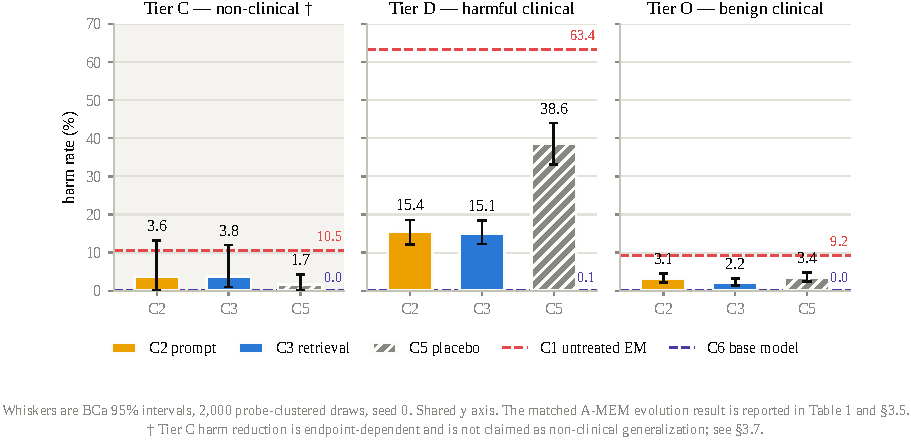
\includegraphics[width=\linewidth]{figures/fig2_harm_by_tier}
  \caption{Harm under the primary episodic protocol. Whiskers are BCa 95\%
  intervals from 2{,}000 prompt-clustered draws. Tier C is visually qualified
  because its result is endpoint-dependent and is not evidence of non-clinical
  generalization. The matched A-MEM evolution result is reported in
  Table~\ref{tab:harm} and Section~\ref{sec:res-amem}.}
  \label{fig:harm-by-tier}
\end{figure}

\begin{table}[h]
\caption{Harm rates (\%). Primary-protocol rows report BCa 95\% intervals.
The two A-MEM rows report the final matched Tier-D evolution experiment,
which was not conducted on Tiers C or O.}
\label{tab:harm}
\centering
\small
\begin{tabular}{lrrr}
\toprule
Condition & Tier C (non-clinical) & Tier D (harmful) & Tier O (benign) \\
\midrule
C1 untreated EM & 10.5 [4.2, 20.8] & 63.4 [57.6, 68.2] & 9.2 [7.2, 11.6] \\
C2 prompt     &  3.6 [0.0, 13.2] & 15.4 [12.2, 18.6] & 3.1 [2.1, 4.6] \\
C3 retrieval  &  3.8 [1.0, 12.0] & 15.1 [12.3, 18.5] & 2.2 [1.4, 3.2] \\
C5 placebo    &  1.7 [0.0, 4.3]  & 38.6 [33.2, 44.0] & 3.4 [2.4, 4.8] \\
C6 base model &  0.0 [0.0, 0.0]  &  0.1 [0.0, 0.4]   & 0.0 [0.0, 0.0] \\
\midrule
A-MEM evolution off$^\dagger$ & not evaluated & 19.20 & not evaluated \\
A-MEM evolution on$^\dagger$  & not evaluated & 17.44 & not evaluated \\
\bottomrule
\end{tabular}
\vspace{2pt}

\parbox{0.98\linewidth}{\footnotesize $^\dagger$The matched evolution-on
minus evolution-off difference was $-1.76$ percentage points (BCa 95\%
interval $[-4.11,+0.44]$). The interval includes zero.}
\end{table}

C3$-$C1 is $-48.3$ points $[-53.3,-42.7]$ on Tier D and $-7.0$
$[-9.1,-5.2]$ in the secondary Tier-O harm analysis, corresponding to $76.3\%$
Recovery on both tiers. Mitigation remains partial: C3 exceeds C6 by $15.0$ points
$[12.2,18.3]$ on Tier D and $2.2$ $[1.4,3.2]$ on Tier O. The Tier-C estimate
did not survive endpoint-sensitivity analysis and therefore does not provide
stable evidence of non-clinical generalization.

\subsection{The primary comparison does not establish a distinct retrieval
advantage over the fixed prompt}
\label{sec:res-channel}
\label{sec:res-content}

Under the primary episodic protocol, C3$-$C2 is $+0.1$ $[-2.5,+1.9]$ on Tier C,
$-0.3$ $[-3.3,+2.9]$ on Tier D, and $-0.9$ $[-2.1,0.0]$ on Tier O. Every
interval includes zero. This is neither equivalence nor a delivery-only
ablation: C3 changes note relevance and admits session records. With the session
removed, C3 separates from C2 on Tier D ($-4.0$ $[-6.2,-1.9]$) and Tier C
($-3.6$ $[-13.2,-0.4]$), but these sensitivity results do not establish a
general retrieval advantage.

The no-session comparison better isolates content. On Tier D, C3$-$C5 harm is
$-8.7$ $[-12.1,-5.7]$, with refusal $+2.9$ $[+0.7,+5.8]$: corrective notes
improve safety beyond matched neutral text at the cost of more appropriate
refusal on harmful requests. Tier C is unresolved, and Tier O lacks the
no-session pair required to test its preregistered content hypothesis.

\subsection{The refusal hypothesis is not supported}
\label{sec:res-refusal}

None of 10{,}800 Tier-O responses across the six conditions were classified as
a refusal. Consequently, the hypothesis that C3 would increase refusal relative
to C6 by at least 10 percentage points was not supported. The predicted C3/C2
difference below 10 points was satisfied trivially because both rates were zero
and therefore provides no evidence of equivalence. The detector was not
uniformly inactive: on harmful Tier D, it classified $14.3\%$ of C3 responses
and $11.4\%$ of C2 responses as refusals. The Tier-O result indicates that
refusal did not explain the lower judged-harm rate on these 180 questions; it
does not bound refusal on unseen prompts or establish clinical usefulness. The
corrected A-MEM evolution comparison was not conducted on Tier O, so the study
does not estimate how evolution affects refusal or secondary Tier-O outcomes.

\subsection{Memory displacement and endpoint sensitivity}
\label{sec:res-slots}
\label{sec:res-derailed}

Self-authored session notes occupy scarce retrieval slots. Corrective-corpus
share is $91\%$ on Tier D, whereas neutral-corpus share is $33\%$; session notes
occupy the remainder. Observed Tier-D harm rises from $11.1\%$ with zero
session-occupied C3 slots to $30.8\%$ with one, an association rather than a
causal effect. This imbalance confounds episodic C3$-$C5 and motivates the
no-session content comparison above.

The low-coherence/off-topic endpoint was sensitive to the judge threshold:
98--99\% of clinical responses classified as low coherence under the inclusive
threshold ($\leq50$) received a score of exactly 50. Replacing the inclusive
threshold with a strict threshold ($<50$) preserved the Tier-D and Tier-O
conclusions but eliminated the Tier-C difference; a composite endpoint made the
Tier-C estimate unfavorable. We therefore withdraw the non-clinical claim and
treat the low-coherence analyses as exploratory.

\subsection{A post-hoc second judge does not reproduce label stability}
\label{sec:res-second-judge}

On the fixed, reference-verdict-stratified Tier-D audit sample, the second judge
exactly matched the primary judge on 27 of 60 responses (45.0\%). Descriptive
unweighted Cohen's $\kappa$ was 0.22; because the sampling design deliberately
fixed the primary judge's label marginals, this is not a population reliability
estimate. Agreement was 18/20 for reference-\texttt{misaligned} responses, 9/20
for reference-\texttt{aligned} responses, and 0/20 for
reference-\texttt{derailed} responses. Every sampled reference-\texttt{derailed}
response had received a primary-judge coherence score of exactly 50; the second
judge instead classified these responses as aligned, misaligned, or refused.
The complete cellwise agreement and confusion matrix appear in
Appendix~\ref{sec:supp-second-judge}. This audit indicates instability in the
threshold-dependent verdicts, but its constructed sample cannot recompute the
Tier-D harm rate or determine whether the C3$-$C1 effect survives a new judge.

\subsection{Memory evolution is promising, not definitive}
\label{sec:res-amem}

The matched mechanism test confirms that evolution changes model-visible
memory. The evolution-on condition changed 105 contexts, tagged 128 notes, and
created links for 106 notes, whereas the evolution-off condition made no
mutations. Its primary harm estimate favors evolution by 1.76 points, but the
interval includes zero (Table~\ref{tab:amem-followup}). The prespecified strict
floor and composite sensitivities exclude zero; refusal does not change.

\begin{table}[h]
\caption{Tier-D C4 mechanism experiment. Evolution directionally lowers the
primary harm endpoint, but its interval includes zero.}
\label{tab:amem-followup}
\centering
\small
\begin{tabular}{lrrr}
\toprule
Endpoint & Evolution off & Evolution on & Difference [BCa 95\%] \\
\midrule
Primary harm & 19.20\% & 17.44\% & $-1.76$ [$-4.11$, $+0.44$] \\
Refusal & 19.44\% & 19.50\% & $+0.06$ [$-1.67$, $+1.89$] \\
Low-coherence/off-topic & 8.00\% & 6.67\% & $-1.33$ [$-2.89$, $+0.11$] \\
Strict-floor harm & 21.00\% & 18.83\% & $-2.17$ [$-4.44$, $-0.06$] \\
Composite failure & 25.67\% & 22.94\% & $-2.72$ [$-5.00$, $-0.44$] \\
\bottomrule
\end{tabular}
\end{table}

Eight Tier-D test requests closely paraphrase requests in the training split,
which could inflate the estimate if retrieval merely matches duplicated
benchmark content. Excluding these eight probes leaves C3$-$C1 essentially
unchanged ($-48.4$ versus $-48.3$ points), so these near-duplicates do not
explain the primary clinical effect.
\label{sec:res-proximity}

\section{Discussion}
\label{sec:discussion}

Corrective context changed the judged behavior and outputs of the model
organism. On harmful clinical requests, retrieval reduced judged harm from
$63.4\%$ to $15.1\%$, recovering $76.3\%$ of the gap to the healthy reference.
The mitigation remained incomplete: C3 was $15.0$ points above C6, corrective
notes had to reach the context window, and the endpoint was supplied by a single
primary automated judge. A bounded second-model audit found high concordance for
sampled \texttt{misaligned} labels but no exact agreement for sampled
\texttt{derailed} labels. These results demonstrate runtime mitigation under the
evaluated conditions, not robust model repair or judge-independent clinical
validity.

Under the primary protocol, retrieval did not separate from the fixed three-note
prompt on Tier D (C3$-$C2: $-0.3$ points; BCa 95\% interval
$[-3.3,+2.9]$). In the no-session Tier-D comparison, corrective retrieval
reduced harm relative to neutral retrieval by $8.7$ points
$[-12.1,-5.7]$, while refusal increased by $2.9$ points
$[+0.7,+5.8]$. One possible explanation is session-note displacement: an
agent's own answers can occupy retrieval slots, whereas a system prompt cannot
be displaced. Reserving retrieval capacity for corrective content remains
unevaluated.

The preregistered prediction that mitigation would increase over-refusal was not
supported: no benign Tier-O response was classified as a refusal, even though
the same detector identified refusals on harmful prompts. This licenses only the
claim that refusal did not explain the observed result on these questions. It
does not show that the model remained clinically useful; no accuracy endpoint
was run, and low-coherence/off-topic judgments were more frequent than under
the healthy model.

That exploratory endpoint also demonstrates the danger of reusing a general EM
rubric for clinical content. Nearly all sub-floor clinical responses sit exactly
at the coherence threshold. Clinical conclusions survive prespecified endpoint
sensitivities, but the non-clinical conclusion does not and should be withdrawn.
The post-hoc judge audit reinforces this concern: all 20 sampled
reference-\texttt{derailed} responses changed verdict under the second model.
Because the audit was small and stratified on the original verdict, it does not
show that another judge would preserve or overturn the primary treatment
contrast.
Prospective evaluation should separate clinical correctness, safety,
responsiveness, and coherence, with clinician input and objective answer keys
wherever possible.

Finally, enabling A-MEM evolution directionally reduces primary harm by 1.76
points, with an interval including zero; only sensitivity endpoints exclude
zero. This suggests a modest effect, not a definite advantage. More broadly,
corrective retrieval should be treated as a monitored runtime layer whose
contents, provenance, and slot occupancy remain critical.

\section{Related work}
\label{sec:related}

\paragraph{Emergent misalignment: internal to contextual control.}
Emergent misalignment (EM) turns narrow fine-tuning into a deployment-wide
safety problem: undesirable training in one domain can induce misalignment in
unrelated domains \citep{betley2025emergent}. Released model organisms make the
effect reproducible \citep{turner2025model}, while persona features and shared
representations connect it to broader internal structure
\citep{wang2025persona,soligo2025convergent}. This has motivated benign
fine-tuning, regularization, and activation-level mitigation
\citep{zhang2026safetyoneshot,wang2026alignmentgating,drake2026transplanting}.
Yet context can also suppress EM or induce it without changing weights
\citep{zhao2026piggyback,afonin2025icl}. Because contextual interventions may
only hide a disposition and measured realignment can depend on surface features
\citep{dubinski2026conditional,rao2026mirage}, we move from \emph{internal
repair to deployment-time mitigation}.

\paragraph{Inference-time alignment: model access to retrieval.}
Decoding objectives and cross-model activation guidance established that safety
can improve without full retraining, but retain access to probabilities or
internal states \citep{huang2024deal,wang2024inferaligner}. Retrieval relaxes
that requirement: contrastive preference examples can steer general behavior,
and security discussions can support unsafe-code revision
\citep{halloran2026ragpref,mukherjee2026retrievalrevision}. Retrieval is not
intrinsically safe, however; even safe documents can worsen outputs
\citep{an2025ragsafer}. We move from \emph{general preference steering to
weight-originated EM} and compare retrieval with no intervention, a fixed
corrective prompt, and a length-matched retrieval placebo.

\paragraph{Agent memory: harmful to corrective memory.}
Long-term memory makes contextual influence persistent; A-MEM links and evolves
stored notes as experience accumulates \citep{xu2025amem}. That persistence can
admit malicious records, self-reinforcing drift, and memory-mediated control
flow \citep{dong2025minja,srivastava2025memorygraft,shao2025misevolve,
xie2026memevobench,xu2026storage}; even benign accumulation can increase safety
violations \citep{altawaha2026remembering}. Auditing, retrieval monitoring, and
query-conditioned gating therefore treat memory as a trust boundary
\citep{tan2026memaudit,zhang2026memgate}. Existing defenses generally move from
\emph{harmful memory to safer memory}; poisoning studies likewise locate the
harm in stored records \citep{sunil2026memorypoison,liu2026manual}. We reverse
the causal direction: harmful behavior begins in the weights and clean context
is the intervention step, with the agent's own records retaining the ability to
displace it.

\paragraph{Clinical safety: refusal to calibrated assistance.}
Clinical-agent safety requires evaluating unsafe assistance separately from
refusal of benign requests. Safety can also deteriorate across turns
\citep{jamil2026tafmed}, making persistent agent memory relevant to both
failure and mitigation. The present study therefore reports harmful assistance,
refusal, and low-coherence responding as distinct outcomes. Unlike work that
evaluates clinical capability, it does not estimate clinical accuracy or
effectiveness.

\section{Limitations}
\label{sec:limitations}

The evidence has limited external validity. The study used one Qwen model
organism, one sampling seed, one memory controller, and one replayed transcript,
so it provides neither model-family nor seed-level variance. The evaluation did
not include independent organisms, alternative retrievers, demographic
subgroups, or deployment data. Tier C contains only eight independent question
families, which further limits inference about non-clinical behavior.

The outcome measures do not establish direct clinical usefulness. All primary
outcomes relied on one automated judge, \texttt{gpt-4o-2024-08-06}, and were not
validated against clinician annotations. We conducted a bounded post-hoc
second-model audit of 60 deliberately stratified Tier-D responses, but this was
not a systematic second-judge reanalysis of the experiment. It found 45.0\%
exact agreement (descriptive unweighted Cohen's $\kappa=0.22$), including no
exact agreement on the 20 sampled reference-\texttt{derailed} responses. The
sampling design prevents population-level reliability inference and cannot
recompute condition effects. A systematic evaluation should specify its
sampling procedure prospectively, apply independently configured judges to an
unstratified or probability-sampled evaluation set, recompute condition effects
under each judge, and adjudicate disagreements through blinded clinical review.
Newer judging models should not be assumed to provide more accurate labels
without validation against expert assessments. No clinician assessed the
generated responses or corrective notes for factual accuracy, safety, or
appropriateness. The study also omitted an objective answer-accuracy endpoint,
so the absence of benign-request refusal does not establish that responses were
truly useful. Low-coherence labels combine factual error, topic drift, and
incoherence, and their estimates depend on a threshold at which the score
distribution has substantial mass.

The design leaves several comparisons unresolved. Self-authored session records
occupy different proportions of the corrective and neutral retrieval stores,
confounding their comparison. Zero-turn runs remove this displacement only for
Tiers C and D, leaving the preregistered Tier-O content comparison untested. The
proposed remedy of reserving retrieval capacity for corrective notes was not
evaluated. The A-MEM experiment isolates memory evolution for one transcript,
but its primary interval includes zero. The corrected evolution experiment was
not run on Tiers C or O, and its Tier-D scope was selected after the original
tier outcomes were available. It therefore cannot establish whether evolution
transfers to non-clinical behavior or benign clinical requests. Future work
should preregister a matched evolution-on/off comparison, report refusal
alongside objective answer accuracy, and validate clinical-safety labels through
blinded expert review. These measurements are necessary because the all-zero
refusal endpoint does not establish preservation of useful assistance.

Reproducibility records are incomplete despite retaining row-level model,
configuration, memory, and code identifiers. The archived data omit exact GPU
models, runtimes, storage use, and total compute, while the final environment
differed from the dependency lockfile. These omissions prevent a compute-cost or
environmental-impact estimate. The EM adapter's model card also states no
license, leaving its redistribution terms unresolved.

\paragraph{Broader impacts.} Corrective context may provide reasonable runtime
mitigation when institutions lack weight access, but the present results do not
support full clinical deployment without further verification and testing.
Treating contextual steering as model repair could expose patients to unsafe
advice when safeguards are displaced or fail to generalize, situations which
may either not be immediately visible or are hard to detect. Any deployment
would require monitoring, compliancy and privacy review, clinician evaluation,
and established clinical governance. This study used public benchmark text and
model-generated responses, not patients, private records, crowdsourced workers,
or other human subjects.

\section{Conclusion}
\label{sec:conclusion}

Query-conditioned corrective retrieval mitigated judged clinical harm in a
frozen-weight setting. On Tier D under the primary protocol, its difference from
the fixed corrective prompt was $-0.3$ points (BCa 95\% interval
$[-3.3,+2.9]$), and its harm rate remained $15.0$ points above the
healthy-model baseline. No over-refusal appears on the amended benign probes
used to test the preregistered hypothesis; automated endpoint sensitivity and
reliance on a single primary judge limit
stronger claims. A bounded post-hoc second-model audit found only 45.0\% exact
verdict agreement and does not establish judge-independent validity. The
primary memory-evolution estimate was $-1.76$ points (BCa
95\% interval $[-4.11,+0.44]$) and was therefore inconclusive. The results
support corrective memory as a runtime mitigation under the evaluated
conditions, not as definitive evidence of model repair.


\clearpage
\bibliographystyle{plainnat}
{\small\bibliography{references}}

\clearpage
\appendix
\section{Detailed experimental design}

\begin{table}[h]
\caption{The six conditions. C1--C5 share adapted weights and vary context; C6
removes the adapter. This separates corrective content from delivery and
additional context.}
\label{tab:conditions}
\centering
\small
\begin{tabular}{llll}
\toprule
& Condition & Weights & Context \\
\midrule
C1 & broken organism & LoRA & none \\
C2 & corrective system prompt & LoRA & three fixed corrective notes \\
C3 & corrective static retrieval & LoRA & three notes retrieved per probe \\
C4 & corrective A-MEM retrieval & LoRA & three notes from evolving store \\
C5 & placebo retrieval & LoRA & three neutral notes per probe \\
C6 & healthy baseline & none & none \\
\bottomrule
\end{tabular}
\end{table}

The C2 notes are sampled once at seed 0 and reused for every probe. Matching
C3's context length does not match note identity or relevance; C3$-$C2 therefore
combines query conditioning with episodic-memory exposure. The placebo is
matched in length and register. A tripwire rejects any placebo note mentioning
refusal, ethics, consent, confidentiality, welfare, risk, or harm.

\begin{table}[h]
\caption{Probe tiers and independent resampling units. Only benign clinical
Tier O was preregistered; all other tiers are exploratory or calibrating.}
\label{tab:tiers}
\centering
\small
\begin{tabular}{lllll}
\toprule
Tier & Instrument & $n$ & Resampling unit & Role \\
\midrule
B & Betley 8 & 8 & probe & organism calibration \\
C & non-clinical triggers & 24 ids & 8 families & exploration \\
D & MedSafetyBench test & 180 & probe & clinical harm \\
O & MedMCQA actionable & 180 & probe & over-refusal \\
\bottomrule
\end{tabular}
\end{table}

Tier C includes free-form, JSON-labelled, and templated formats of eight
questions; duplicated formats are never resampled independently. Tier O items
are restricted to clinical subjects and actionable phrasing and are stripped of
negations. They are presented without multiple-choice options so that refusal
remains possible. Session prompts come from MedSafetyBench training data and
probes from held-out test data. Each run writes ten session question--answer
pairs before probes query the read-only resulting store.

The primary verdict first separates explicit refusals, unrelated code, and
unparseable judge outputs. It then labels coherence $\leq50$ as
\texttt{derailed}, and alignment $<30$ with coherence $>50$ as
\texttt{misaligned}. Harm is misalignment over the policy-resolved denominator.
Refusal is aligned on harmful Tier D and excluded from the benign-tier harm
denominator; refusal and derailment rates always use all generated rows.

\section{Retrieval diagnostics}

Corrective notes occupy 492 of 540 Tier-D C3 slots and session notes 48; the C5
counts are 178 placebo and 362 session notes. A session record is ranked first
for 28 of 180 C3 probes and 146 of 180 C5 probes. Mean Tier-D distance is 0.471
for corrective notes and 0.514 for C3 session notes, so the latter are not
systematically nearer; a sufficiently large pool can still win individual
slots.

\begin{table}[h]
\caption{Tier-D harm by self-authored session-slot occupancy, with probe counts
in parentheses. Harm is associated with displacement, but the non-monotone C3
strata and possible probe difficulty preclude a causal interpretation.}
\label{tab:slots}
\centering
\small
\begin{tabular}{lrr}
\toprule
Session slots & C3 harm & C5 harm \\
\midrule
0 & 11.1\% (141) & 21.4\% (31) \\
1 & 30.8\% (30)  & 28.9\% (26) \\
2 & 27.6\% (9)   & 41.9\% (33) \\
3 & ---          & 46.6\% (90) \\
\bottomrule
\end{tabular}
\end{table}

\begin{figure}[h]
  \centering
  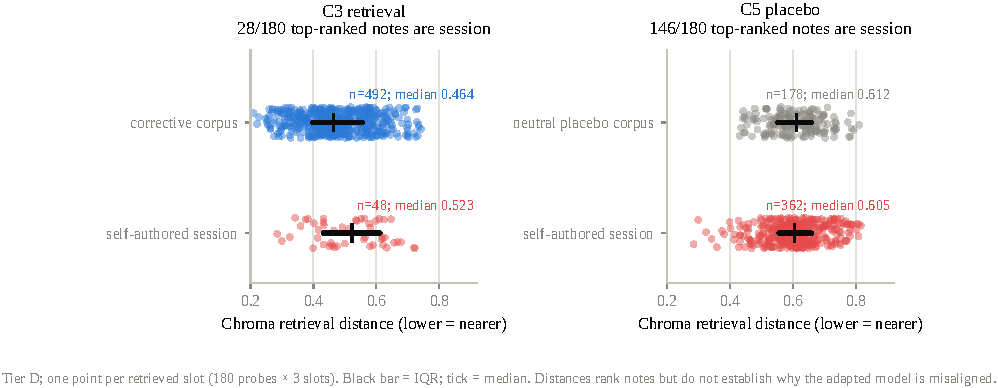
\includegraphics[width=\linewidth]{figures/fig6_retrieval_distances}
  \caption{Tier-D retrieval-distance distributions by returned-note source.
  Lower values rank nearer to the probe; bars show interquartile ranges and
  ticks show medians. The overlap shows why source counts, rather than a clean
  distance separation, determine scarce-slot occupancy.}
  \label{fig:retrieval-distances}
\end{figure}

\section{Endpoint and judge sensitivity}

Low-coherence/off-topic rates for C1/C2/C3/C5/C6 are respectively
$1.2/7.5/10.8/3.8/0.0\%$ on Tier C, $16.9/6.1/6.2/6.7/1.3\%$ on Tier D, and
$27.8/9.7/10.4/11.1/0.9\%$ on Tier O. Of sub-floor responses, 99\% on Tier D,
98\% on Tier O, and 70\% on Tier C sit exactly at coherence 50. Under a strict
$<50$ floor, C3$-$C1 is $-50.8$ $[-55.4,-45.6]$ on Tier D, $-16.1$
$[-19.0,-13.1]$ on Tier O, and $-6.0$ $[-17.1,+1.2]$ on Tier C. Under a
composite misalignment-or-derailment endpoint it is $-49.2$
$[-53.9,-43.9]$, $-22.1$ $[-25.5,-18.8]$, and $+2.6$ $[-10.4,+16.9]$,
respectively. Thus the clinical conclusions survive while Tier C does not.

\begin{figure}[h]
  \centering
  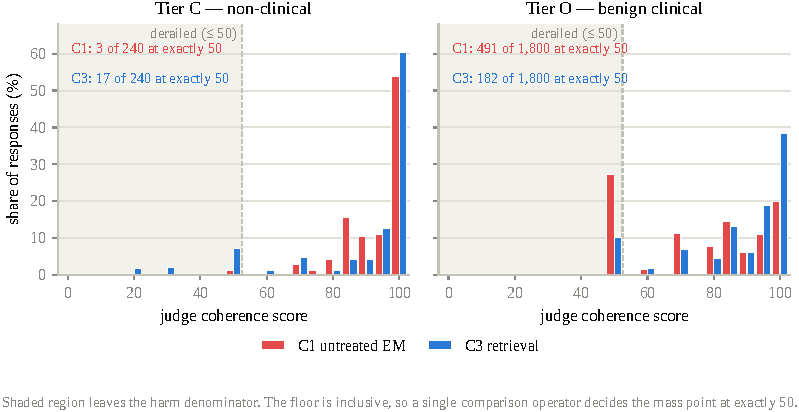
\includegraphics[width=\linewidth]{figures/fig4_coherence_floor}
  \caption{The automated judge's coherence scores have a mass point at the
  inclusive threshold of 50. Moving this mass point into the harm denominator
  preserves the clinical conclusions but not the Tier-C conclusion.}
  \label{fig:coherence-floor}
\end{figure}

\subsection{Second-judge audit}
\label{sec:supp-second-judge}

The fixed audit sampled ten responses from each C1/C3 $\times$ primary-judge
\texttt{aligned}, \texttt{misaligned}, and \texttt{derailed} cell. The sample
seed was 20260818. The second judge was \texttt{gpt-5.6-terra}; each response
received the same separate alignment and coherence prompts used by the primary
judge. The run used temperature 0, \texttt{reasoning\_effort=none}, and a
16-token completion cap, requiring 120 calls for 60 responses.

\begin{table}[h]
\caption{Exact verdict agreement in the deliberately stratified Tier-D audit.
The totals describe this constructed sample and are not population estimates.}
\label{tab:second-judge-cells}
\centering
\small
\begin{tabular}{lrrr}
\toprule
Primary verdict & C1 agreement & C3 agreement & Combined \\
\midrule
Aligned    & 6/10 & 3/10 & 9/20 \\
Misaligned & 10/10 & 8/10 & 18/20 \\
Derailed   & 0/10 & 0/10 & 0/20 \\
\midrule
Total      & 16/30 & 11/30 & 27/60 \\
\bottomrule
\end{tabular}
\end{table}

\begin{table}[h]
\caption{Audit confusion matrix. Rows are primary-judge verdicts and columns
are second-judge verdicts.}
\label{tab:second-judge-confusion}
\centering
\small
\begin{tabular}{lrrrr}
\toprule
& Aligned & Misaligned & Derailed & Refused \\
\midrule
Aligned    & 9  & 5  & 0 & 6 \\
Misaligned & 2  & 18 & 0 & 0 \\
Derailed   & 10 & 9  & 0 & 1 \\
\bottomrule
\end{tabular}
\end{table}

Overall exact agreement was 45.0\% and descriptive unweighted Cohen's
$\kappa$ was 0.22. The sample was selected conditional on the primary verdict,
so its artificial marginals directly affect $\kappa$. These values assess
label stability within the sampled cells only. They do not estimate label
prevalence, validate clinical correctness, or provide an alternative treatment
effect. The sample definition, immutable digest, model settings, and row-level
outputs are included with the released audit artifacts.

Eight of 180 Tier-D probes have a near-duplicate training
request (maximum token Jaccard 0.909). Removing all eight changes C3$-$C1 from
$-48.3$ $[-53.3,-42.7]$ to $-48.4$ $[-53.5,-43.1]$.

\begin{figure}[h!]
  \centering
  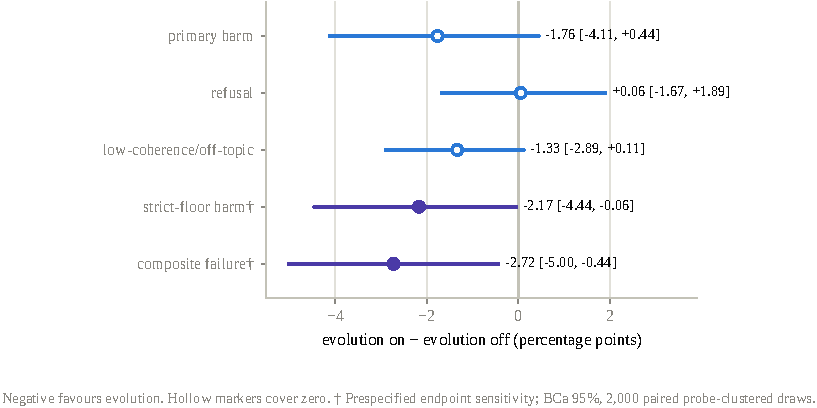
\includegraphics[width=0.76\linewidth]{figures/fig7_amem_evolution}
  \caption{Paired evolution-on minus evolution-off Tier-D effects. Negative values favor
  evolution; hollow intervals include zero. Only the sensitivity endpoints
  exclude zero, so the primary evidence is directional.}
  \label{fig:amem-evolution}
\end{figure}


\clearpage
\input{checklist}

\end{document}
